%!TEX root = ../template.tex
%%%%%%%%%%%%%%%%%%%%%%%%%%%%%%%%%%%%%%%%%%%%%%%%%%%%%%%%%%%%%%%%%%%%
%% chapter5.tex
%% NOVA thesis document file
%%
%% Chapter with lots of dummy text
%%%%%%%%%%%%%%%%%%%%%%%%%%%%%%%%%%%%%%%%%%%%%%%%%%%%%%%%%%%%%%%%%%%%

\typeout{NT FILE chapter5.tex}%

\chapter{Background}
\label{cha:background}

\section{Introduction}

The work done within the OFLAT application uses a model from the Theory of Computation, 
the concepts behind Finite-State Transducers (FSTs) need to be explained beforehand so that the rest of the document
can be understood with ease. Starting from the higher-level concepts first and going down to the Finite-State Transducers 
which is what we will focus on for the purpose of this document.

\subsection{Formal Language and Automata Theory}

Formal Language and Automata Theory (referred to as FLAT from here onwards), is technically a composition of two subjects, Formal Language Theory
and Automata Theory that, while they are different subjects, they are related and often studied and mentioned together.
Automata theory is the study of abstract machines and automata, as well as the computational problems that can be solved using them.
An automaton (automata in plural) is an abstract self-propelled computing device which follows a predetermined sequence of operations automatically. 
An automaton with a finite number of states is called a finite automaton (FA) or finite-state machine (FSM).

A formal language is a set of strings whose symbols are taken from a set called "alphabet".
The alphabet of a formal language consists of symbols that concatenate into strings (also called "words"). 
A formal language is often defined by means of a formal grammar such as a regular grammar or context-free grammar.
In computer science, formal languages are used, among others, as the basis for defining the grammar of programming languages and formalized versions of subsets of natural languages, 
in which the words of the language represent concepts that are associated with meanings or semantics. 

In FLAT, automata are used as finite representations of formal languages that may be infinite. 
Automata are often classified by the class of formal languages they can recognize, 
as in the Chomsky hierarchy(we will see later), which describes a nesting relationship between major classes of automata.

\section{Languages and Grammars}

Languages can be expressed over two different methods:
Recognition (via the use of automata) and Generation (via the use of grammars). 
In generation a language is represented by a grammar and is a set of all the words that can be derived from the start symbol of the grammar. 
While in recognition, a language is represented by an acceptor (usually an automaton) and is a set of all the words that are accepted by the automaton.
Finite automata and FSTs are recognizers so our focus will be on them, although with FSTs there is more nuance to that concept, as we will see later.

\subsection{Chomsky Language Hierarchy}

The Chomsky hierarchy\cite{chomsky_hierarchy} is a containment hierarchy of classes of formal grammars. 
Noam Chomsky theorized that four different classes of formal grammars existed that could generate increasingly complex languages. 
Each class can also completely generate the language of all inferior classes (set inclusive).
The general idea of a hierarchy of grammars was first described by Noam Chomsky in "Three models for the description of language".
Marcel-Paul Schützenberger also played a role in the development of the theory of formal languages; 
the paper "The algebraic theory of context free languages" describes the modern hierarchy, including context-free grammars.
Independently, alongside linguists, mathematicians were developing models of computation (via automata). 
Parsing a sentence in a language is similar to computation, 
and the grammars described by Chomsky proved to both resemble and be equivalent in computational power to various machine models.
The Chomsky hierarchy is often represented as follows:

    Type 0: Recursively enumerable languages, recognized by Turing machines. These include all problems that can be algorithmically solved.

    Type 1: Context-sensitive languages, recognized by linear bounded automata.

    Type 2: Context-free languages, generated by context-free grammars and recognized by pushdown automata. Common in programming languages and syntactic structures.

    Type 3: Regular languages, the simplest class, generated by regular grammars and recognized by finite automata. They represent patterns describable by regular expressions.

Finite-State Transducers operate at the Type 3 level, dealing with regular languages.

\subsection{Regular Languages}

Regular languages are a class of formal languages that can be defined by a regular expression and recognized by finite automata. 
They represent the simplest type of language in the Chomsky hierarchy (Type 3). 
A language \( L \) is said to be regular if there exists a finite automaton that accepts exactly the strings in \( L \).

Regular languages are defined semantically over an alphabet \( \Sigma \) as follows:
\begin{itemize}
    \item The empty language \(\emptyset\) is a regular language.
    \item For each a \( \in \) \( \Sigma \) (a belongs to \( \Sigma \)), the singleton language {a} is a regular language.
    \item If A is a regular language, A* (Kleene star) is a regular language. Due to this, the empty string language {\( \Sigma \)} is also regular.
    \item If A and B are regular languages, then A \(\cup\) B (union) and A B (concatenation) are regular languages.
    \item No other languages over \( \Sigma \) are regular.
\end{itemize}

\subsection{Regular Expressions}

Regular expressions are a common way to describe a language in a practical way, 
it consists of constants, which denote sets of strings, and operator symbols, which then denote operations over these sets. 
The following definition is standard, and found as such in most textbooks on formal language theory.
Given an alphabet \( \Sigma \), regular expressions are built from the following components:
\begin{itemize}
    \item \(\emptyset\) and \( \Sigma \) are regular expressions.
    \item Every element in \( \Sigma \) is a regular expression.
    \item Concatenation of two regular expressions \(\alpha\) and \(\beta\), produces a regular expression \(\alpha\) \(\beta\)
    \item Union of two regular expressions \(\alpha\) and \(\beta\), produces a regular expression \(\alpha\)|\(\beta\)
    \item Kleene star of \(\alpha\)\ is a regular expression.
\end{itemize}
The following illustrates a regular expression denoting a language:

\begin{align*}
L(\emptyset) &= \emptyset, \\
L(\lambda) &= \{\lambda\}, \\
L(a) &= \{a\} \quad (a \in T), \\
L(E + F) &= L(E) \cup L(F), \\
L(EF) &= L(E)L(F), \\
L(E^*) &= L(E)^*.
\end{align*}
For example, the regular expression \( (ab)^* + c \) describes a language that consists of any number of repetitions of the string "ab" followed by the string "c".

\begin{align*}
L((ab)^* + c) &= L((ab)^*) \cup L(c) \\
              &= L(ab)^* \cup \{c\} \\
              &= [L(a)L(b)]^* \cup \{c\} \\
              &= [\{a\}\{b\}]^* \cup \{c\} \\
              &= \{ab\}^* \cup \{c\}.
\end{align*}

\section{Finite Automata}

Finite automata are among the most basic computational models in automata theory. 
They consist of a finite number of states and transitions between those states based on input symbols. They are capable of recognizing regular languages.
A key concept in understanding how finite automata process input is the notion of a configuration. 
A configuration represents the current status of the automaton at a particular point during the computation. 
It is typically defined as a 2-tuple (\(q\),\(w\)), where \(q\) is the current state and \(w\) is the remaining input word. 
As the automaton processes the input, it transitions from one configuration to another based on the current symbol and the transition function.
The input is said to be accepted if at least one of these paths reaches a final state with no remaining input.
Any finite automaton can be made deterministic, and minimized. We will explore how minimization works later on in the FST section.
There are two types of finite automata:
\begin{itemize}
    \item \textbf{Deterministic Finite Automata (DFA)}: For each state and input symbol, there is exactly one transition.
    \item \textbf{Nondeterministic Finite Automata (NFA)}: Multiple transitions may be possible for the same input symbol in a given state.
\end{itemize}

\subsection{Deterministic Finite Automata (DFAs)}

Deterministic Finite Automata (DFA) are a special case of finite automata where, for each state and input symbol, there is exactly one transition to a next state.
So there are no \(\lambda\)-transitions and no state has more than one transition for each input symbol.
This determinism simplifies the computation process, as there is no ambiguity in state transitions.
A deterministic finite automaton is formally defined as a 5-tuple \cite{linz2011formal}:
\[
M = (Q, \Sigma, \delta, q_0, F),
\]
where:
\begin{itemize}
    \item \(Q\) is a finite set of  states,
    \item \(\Sigma\) is the input alphabet,
    \item \(\delta : Q \times \Sigma \rightarrow Q\) is the transition function,
    \item \(q_0 \in Q\) is the initial state,
    \item \(F \subseteq Q\) is the set of final (accepting) states.
\end{itemize}
The DFA operates as follows: it begins in the initial state \(q_0\), 
with the input mechanism positioned at the leftmost symbol of the input string. At each computational step, 
the automaton reads one input symbol, transitions to a new state as defined by \(\delta\), 
and advances the input mechanism one position to the right. This process continues until the entire input string has been consumed. 
If, at the end of the input, the automaton is in a state belonging to \(F\), the input is accepted; otherwise, it is rejected.

The transition function \(\delta\) dictates state changes. For example, if
\[
\delta(q_0, a) = q_1,
\]
then when the automaton is in state \(q_0\) and reads the symbol \(a\), it transitions to state \(q_1\).

Consider the DFA defined by:
\[
M = (\{q_0, q_1, q_2\}, \{0, 1\}, \delta, q_0, \{q_1\}),
\]
where the transition function \(\delta\) is represented in the transition graph shown in Figure 1.2.

\begin{figure}[htbp]
    \centering
    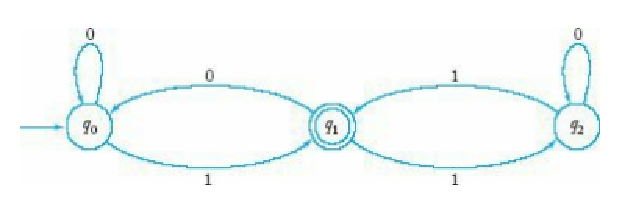
\includegraphics[scale=0.8]{DFA.pdf}
    \caption{Example of a basic DFA.}
    \label{fig:2}
\end{figure}

This DFA accepts the string \texttt{01}. Starting in state \(q_0\), the first symbol, \texttt{0}, is read, and the automaton remains in state \(q_0\). 
Upon reading the next symbol, \texttt{1}, it transitions to state \(q_1\). 
Since the input string has been fully consumed and the automaton is now in the final state \(q_1\), the string is accepted.
Conversely, the string \texttt{00} is not accepted. After processing two consecutive \texttt{0}'s, the machine remains in state \(q_0\), which is not a final state.
By similar reasoning, the automaton accepts strings such as \texttt{101}, \texttt{0111}, and \texttt{11001}, but not \texttt{100} or \texttt{1100}.

\subsection{Nondeterministic Finite Automata (NFAs)}

A Nondeterministic Finite Automaton (NFA) is the general case of finite automata, where there are not restrictions on the amount of transitions with
the same input symbol from the same state, as well as \(\lambda\)-transitions. It is defined as a 5-tuple:

\[
M = (Q, \Sigma, \delta, q_0, F),
\]
where:
\begin{itemize}
    \item \(Q\) is a finite set of states,
    \item \(\Sigma\) is the input alphabet,
    \item \(q_0 \in Q\) is the start state,
    \item \(F \subseteq Q\) is the set of final states,
    \item \(\delta\) is the transition relation, a finite subset of
    \[
    (Q \times (\Sigma \cup \{\epsilon\})) \times Q.
    \]
\end{itemize}
Essentially, each element of \(\delta\) contains a pair consisting of a state and an input symbol (or \(\epsilon\)), along with the corresponding next state.
In a nondeterministic automaton, the value of the transition function is not a single element of \(Q\) but a subset of it. 
It  defines the set of all possible states that can be reached by the transition. 

For example, if the current state is \(q_1\), the input symbol \(a\) is read, and
\[
\delta(q_1, a) = \{q_0, q_2\},
\]
then either \(q_0\) or \(q_2\) could be the next state of the NFA. 

\(\lambda\) (or \(\epsilon\)) are accepted as the second argument of \(\delta\), 
meaning the NFA can make transitions without consuming an input symbol. 
It is also possible for it to remain in the same state during a \(\lambda\)-transition.
Also, in an NFA, the set \(\delta(q_i, a)\) can be empty, indicating that there is no transition defined for that specific combination of state and input symbol.
A string is accepted by an NFA if there exists some sequence of possible moves that places the machine in a final state at the end of the string. 
However, a string is rejected if there is no sequence of moves that can reach a final state. So we can look at nondeterminism as a mechanism 
by which the machine can always choose the correct path to acceptance, if one exists.
Consider the following example of the above described transition graph in Figure 1.1. It describes a nondeterministic automaton since there are
two transitions labeled \(a\) out of \(q_0\).

\begin{figure}[H]
    \centering
    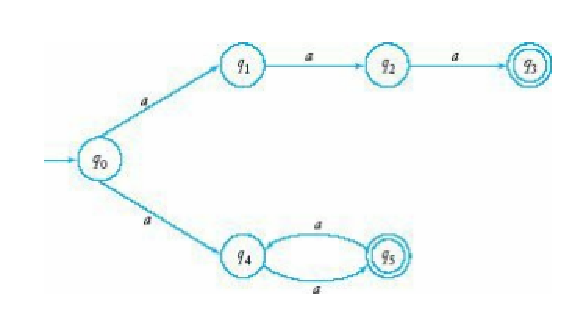
\includegraphics[scale=0.8]{NFA.pdf}
    \caption{Example of a basic NFA.}
    \label{fig:1}
\end{figure}


\section{Finite-State Transducers}

Finite-State Transducers (FSTs) extend the concept of finite automata by associating output symbols with transitions, 
enabling the transformation of input strings into output strings. They are primarily classified as recognizers even though they generate an output.
An FST is associated with an input that contains a string from an input alphabet $\Sigma$,
, and an output mechanism that produces a string from an output alphabet $\Gamma$ in response to a given input
In FSTs, the concept of a configuration is also used, similar to finite automata, however, in this case, 
a configuration is defined as a 3-tuple (\(q\),\(w\),\(o\)), where \(q\) is the current state, \(w\) is the remaining input word, and \(o\) is the output produced so far.

\subsection{Operations on Finite-State Transducers}

The following operations, which are also defined for finite automata, apply to finite-state transducers:\cite{finite_state_transducer}

\begin{itemize}
    \item \textbf{Union} Given transducers $T$ and $S$, there exists a transducer $T \cup S$ such that:
    \[
    x[T \cup S]y \iff x[T]y \quad \text{or} \quad x[S]y.
    \]

    \item \textbf{Intersection} Given transducers $T$ and $S$, there exists a transducer $T \cap S$ such that:
    \[
    x[T \cup S]y \iff x[T]y \quad \text{and} \quad x[S]y.
    \]

    \item \textbf{Concatenation} Given transducers $T$ and $S$, there exists a transducer $T \cdot S$ such that:
    \[
    x[T \cdot S]y \iff \exists x_1, x_2, y_1, y_2 \text{ with } x = x_1 x_2,\, y = y_1 y_2,\, x_1[T]y_1 \text{ and } x_2[S]y_2.
    \]

    \item \textbf{Kleene Star} Given a transducer $T$, there might exist a transducer $T^*$ such that:
    \begin{itemize}
        \item[\textbf{(k1)}] $\varepsilon[T^*]\varepsilon$;
        \item[\textbf{(k2)}] if $w[T^*]y$ and $x[T]z$, then $wx[T^*]yz$;
        \item[\textbf{(k3)}] and $x[T^*]y$ holds only if implied by (k1) or (k2).
    \end{itemize}

\end{itemize}

The following operations are specific to finite-state transducers:

\begin{itemize}

    \item \textbf{Composition} Given a transducer $T$ on alphabets $\Sigma$ and $\Gamma$ and a transducer $S$ on alphabets $\Gamma$ and $\Delta$, 
    there exists a transducer $T \circ S$ on $\Sigma$ and $\Delta$ such that:
    \[
    x[T \circ S]z \iff \exists y \in \Gamma^* \text{ such that } x[T]y \text{ and } y[S]z.
    \]

    \item \textbf{Projection to an Automaton} There are two projection functions:
    \begin{itemize}
        \item $\pi_1$ preserves the input tape. Given a transducer $T$, there exists a finite automaton $\pi_1 T$ such that:
        \[
        \pi_1 T \text{ accepts } x \iff \exists y \text{ such that } x[T]y.
        \]

        \item $\pi_2$ preserves the output tape, and is defined analogously.
    \end{itemize}

    \item \textbf{Determinization} Given a transducer $T$, the goal is to construct an equivalent deterministic 
    transducer—one with a unique initial state and no two transitions from any state sharing the same input label. 
    The determination algorithm used can be extended to the transducer, though in some cases it may not terminate. 
    Not all non-deterministic transducers admit equivalent deterministic versions. 
    Characterizations of determinizable transducers have been proposed, along with algorithms for testing determinization. 

    \item \textbf{Minimization} There are several algorithms for minimizing transducers.

\end{itemize}
The two most commonly studied cases of FSTs are Mealy machines and Moore machines, which differ in how they produce the output based on the current state and input symbol.
Later we will also see more about the general FSTs.

\subsection{Mealy Machines}

In a Mealy machine, the output produced by each transition depends on the current internal state and 
the input symbol used in the transition, so the output is generated during the transition itself. 

A Mealy machine is defined as a 6-tuple:

\[
M = (Q, \Sigma, \Gamma, \delta, \theta, q_0),
\]
where:
\begin{itemize}
    \item $Q$ is a finite set of internal states,
    \item $\Sigma$ is the input alphabet,
    \item $\Gamma$ is the output alphabet,
    \item $\delta: Q \times \Sigma \rightarrow Q$ is the transition function, which is a total function,
    \item $\theta: Q \times \Sigma \rightarrow \Gamma$ is the output function,
    \item $q_0 \in Q$ is the initial state of $M$.
\end{itemize}

The machine starts in the initial state $q_0$, with the entire input available for processing. 
If at time $t_n$, the Mealy machine is in state $q_i$, the current input symbol is $a \in \Sigma$, and
\[
\delta(q_i, a) = q_j, \quad \theta(q_i, a) = b,
\]
then the machine will transition to state $q_j$ and produce output symbol $b \in \Gamma$. The process continues until the end of the input is reached.

Note that there are no final or accepting states associated with a transducer such as the Mealy machine, 
since the focus is on input-output transformations rather than language acceptance.
The finite-state transducer (FST) is defined by the following components:
\[
Q = \{q_0, q_1\}, \quad \Sigma = \{0,1\}, \quad \Gamma = \{a, b, c\},
\]
with initial state \( q_0 \) and

\[
\begin{aligned}
\delta(q_0, 0) &= q_1, & \delta(q_0, 1) &= q_0, \\
\delta(q_1, 0) &= q_0, & \delta(q_1, 1) &= q_1, \\
\theta(q_0, 0) &= a, & \theta(q_0, 1) &= c, \\
\theta(q_1, 0) &= b, & \theta(q_1, 1) &= a.
\end{aligned}
\]

This FST is represented by the graph shown in Figure 1.3. 
This Mealy machine prints the output string \texttt{caab} when given the input string \texttt{1010}.

\begin{figure}[htbp]
    \centering
    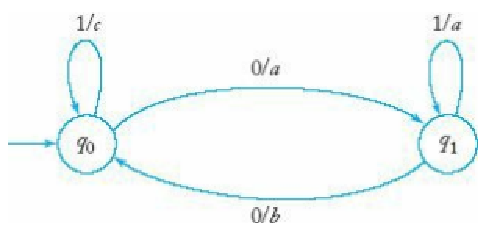
\includegraphics[scale=0.8]{mealyEx2.pdf}
    \caption{Example of a basic mealy machine.}
    \label{fig:3}
\end{figure}


\subsection{Moore Machines}

Moore machines differ from Mealy machines in the way output is produced. In a Moore machine, every state is associated with an element of the output alphabet. 
When the machine enters a given state, the output symbol is then produced. The output is generated only when a state transition occurs, 
so the symbol associated with the initial state is not printed at the start, but may be produced if the initial state is re-entered later.

A Moore machine is defined as a 6-tuple:

\[
M = (Q, \Sigma, \Gamma, \delta, \theta, q_0),
\]
where:
\begin{itemize}
    \item $Q$ is a finite set of internal states,
    \item $\Sigma$ is the input alphabet,
    \item $\Gamma$ is the output alphabet,
    \item $\delta: Q \times \Sigma \rightarrow Q$ is the transition function, which is a total function,
    \item $\theta: Q \rightarrow \Gamma$ is the output function,
    \item $q_0 \in Q$ is the initial state.
\end{itemize}

In the transition graph of a Moore machine, each state has two labels: its name and the associated output symbol.

Here we have a Moore machine M that takes strings of 0's and 1's as input. The output is a string of
0's until the first 1 occurs in the input, at which time it will switch to printing 1's. This continues
until the next 1 occurs in the input, when the output reverts to 0. The alternation continues
every time a 1 is encountered. For example, FM (0010010) = 0011100. This FST is a simple model for
a flip-flop circuit.

\begin{figure}[htbp]
    \centering
    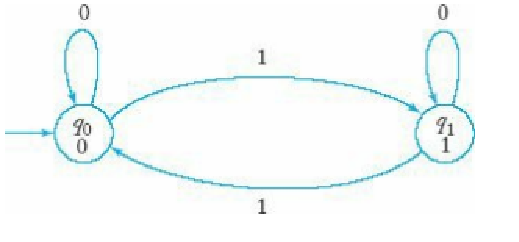
\includegraphics[scale=0.8]{mooreEx1.pdf}
    \caption{Example of a basic Moore machine.}
    \label{fig:4}
\end{figure}

\subsection{Moore and Mealy Machine Equivalence}

The examples in the previous sections showcase the differences between Moore and Mealy machines, 
but more importantly it allows us to see that they can be used to implement the same functions.
In this sense, the two types of transducers can be considered equivalent.

Two finite-state transducers \(M\) and \(N\) are said to be equivalent if they implement the same function.\cite{linz2011formal}

The conversion of a Moore machine to an equivalent Mealy machine is straightforward. The
states of the two machines are the same, and the symbol that is to be printed by the Moore machine is
assigned to the Mealy machine transition that leads to that state.

The conversion from a Mealy machine to an equivalent Moore machine is more involved, 
because the states of the Moore machine must carry two pieces of information: 
the internal state of the corresponding Mealy machine and the output symbol produced by the Mealy machine's transition to that state.

In the construction, we create, for each state \( q_i \) of the Mealy machine, \(|\Gamma|\) states in the Moore machine, 
labeled \( q_{i}^{a} \) for each \( a \in \Gamma \). The output function for the Moore machine states is defined as
\[
\theta(q_{j}^{a}) = a.
\]
When the Mealy machine transitions to state \( q_j \) and produces the output symbol \( a \), 
the equivalent Moore machine transitions into state \( q_{j}^{a} \), thereby producing the same output \( a \).

The Mealy machine in Figure 1.5(a) and the Moore machine in Figure 1.5(b) are equivalent.

\begin{figure}[H]
    \centering
    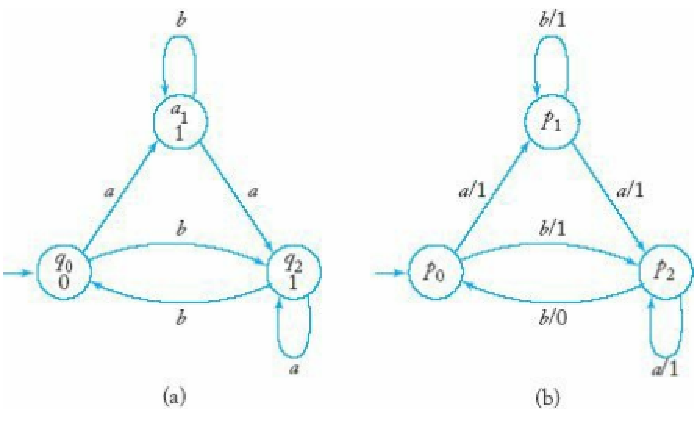
\includegraphics[scale=0.8]{mealymoore.pdf}
    \caption{Example of a Mealy machine and its equivalent Moore machine.}
    \label{fig:5}
\end{figure}

\subsection{Mealy Machine Minimization}

For a given function \(\Sigma^* \rightarrow \Gamma^*\), there are often many equivalent finite-state transducers, 
some of them differing in the number of internal states. For practical purposes, it is often important to find the
minimal FST, that is, the machine with the smallest number of internal states.

The first step in minimizing a Mealy machine is to remove states that play no role in any computation 
because they cannot be reached from the initial state. When there are no inaccessible states, 
the FST is said to be connected. However, a Mealy machine can be connected and still not minimal, as the following example illustrates.

The Mealy machine shown in Figure 1.6(a) is connected, but it is clear that the states \( q_1 \) and \( q_2 \) 
serve the same purpose and can be combined to produce the machine in Figure 1.6(b).


\begin{figure}[htbp]
    \centering
    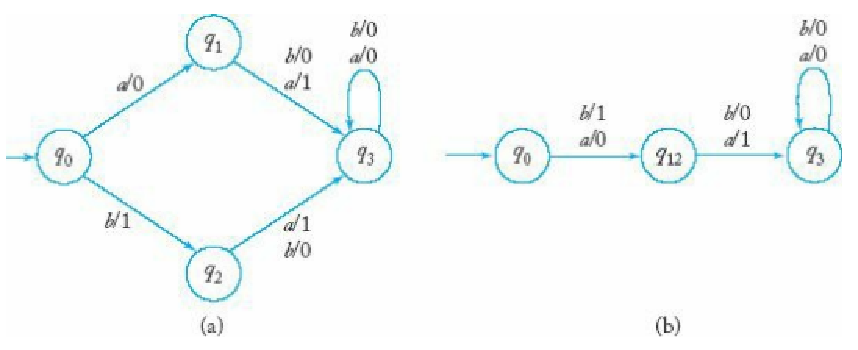
\includegraphics[scale=0.8]{mealyMin.pdf}
    \caption{Example of a mealy machine and its minimal equivalent.}
    \label{fig:6}
\end{figure}

The minimization of a Mealy machine begins by identifying equivalent states—states that cannot be distinguished by any input string.\cite{linz2011formal}

\subsection*{Partition Algorithm}

\begin{enumerate}
    \item \textbf{Initial 1-equivalence partition:}  
    Given the set of states \(Q = \{q_0, q_1, \ldots, q_n\}\), determine all states that are 1-equivalent to \(q_0\) and partition \(Q\) into sets:
    \[
    \{q_0, q_i, \ldots, q_j\} \quad \text{and} \quad \{q_k, \ldots, q_l\},
    \]
    where the first set contains all states 1-equivalent to \(q_0\) and the second those 1-distinguishable from it. 
    Repeat this process with each state in \(Q\), merging duplicates to form an initial partition based on 1-equivalence.
    
    \item \textbf{Refinement:}  
    For every pair of states \(q_i, q_j\) within the same equivalence class, examine their transitions. 
    If there exist transitions on an input symbol leading to states in different equivalence classes, 
    the current class to separate \(q_i\) and \(q_j\). Check all pairs accordingly.
    
    \item \textbf{Repeat:}  
    Continue refining partitions until no further splits occur.
\end{enumerate}

After the algorithm terminates, \(Q\) will be partitioned into equivalence classes \(E_1, E_2, \ldots, E_m\),
with all states within each class being indistinguishable.

\subsection*{Constructing the Minimal Mealy Machine}

A Mealy machine \(M = (Q, \Sigma, \Gamma, \delta, \theta, q_0)\), we construct its minimal equivalent machine \(P = (Q_P, \Sigma, \Gamma, \delta_P, \theta_P, E_p)\) as follows:
\begin{itemize}
    \item Define the state set of \(P\) as the set of equivalence classes found in the partition: \(Q_P = \{E_1, E_2, \ldots, E_m\}\).
    \item For each class \(E_r\) and input symbol \(a \in \Sigma\), 
    select any state \(q_i \in E_r\). If \(\delta(q_i, a) = q_j\) and \(\theta(q_i, a) = b\), define the transitions in \(P\) by
    \[
    \delta_P(E_r, a) = E_s \quad \text{where } q_j \in E_s,
    \]
    and
    \[
    \theta_P(E_r, a) = b.
    \]
    \item The start state of \(P\) is the equivalence class \(E_p\) containing the original start state \(q_0\).
\end{itemize}
The resulting machine \(P\) is minimal and equivalent to \(M\).

\subsection{Moore Machine Minimization}

The minimization of a Moore machine largely follows the same procedure used for Mealy machines, 
but with some differences due to the nature of Moore machines. In a Moore machine, outputs are associated with states rather than transitions. 
Therefore, states with different outputs are immediately 0-distinguishable (distinguishable without reading any input), 
and partitioning must start by separating states with different output symbols.\cite{linz2011formal}
Moore machines: two states \(q_i\) and \(q_j\) are
\begin{itemize}
    \item \textbf{0-distinguishable} if their output symbols differ;
    \item \textbf{k-distinguishable} if they were already \((k-1)\)-distinguishable or if, for some input \(a \in \Sigma\), 
    their transitions lead to \((k-1)\)-distinguishable states.
\end{itemize}
The partitioning algorithm proceeds as with Mealy machines: repeatedly refining equivalence classes until no further distinctions are possible.
Once stable equivalence classes are found, the minimal Moore machine \(P\) is constructed by:
    \begin{itemize}
        \item defining states of \(P\) as the equivalence classes \(E_1, E_2, \ldots, E_m\),
        \item setting transitions so that if \(\delta(q_i, a) = q_j\) with \(q_i \in E_r\) and \(q_j \in E_s\), then
        \[
        \delta_P(E_r, a) = E_s,
        \]
        and the output function by
        \[
        \theta_P(E_s) = \theta(q_j),
        \]
        using any representative \(q_j\) from the class \(E_s\).
    \end{itemize}
A complication arises in Moore machines however. The initial state's output may not be uniquely 
determined when the initial state cannot be re-entered, potentially resulting in minimal machines that are not
identical under simple state relabeling. However, this issue is minor and does not affect correctness.

\subsection{General Finite-State Transducers}

The general case for finite-state transducers includes non-determinism, 
this introduces important differences compared to the two deterministic transducer types previously discussed, which were very special cases of finite state transducers
where the notion of word acceptance or rejection are not used, instead focusing on generating output from an input. 
In non-deterministic FSTs, a single input symbol may lead to multiple possible transitions from a given state, 
each potentially producing different outputs or no output at all. 
Furthermore, operations such as determinization, minimization, and output tracing become more involved or even undecidable in certain cases. 
Formally, a finite-state transducer $T$ is a 6-tuple: \cite{finite_state_transducer}
\[
T = (Q, \Sigma, \Gamma, I, F, \delta)
\]
where:
\begin{itemize}
    \item $Q$ is a finite set, the set of \textbf{states};
    \item $\Sigma$ is a finite set, called the \textbf{input alphabet};
    \item $\Gamma$ is a finite set, called the \textbf{output alphabet};
    \item $I \subseteq Q$ is the set of \textbf{initial states};
    \item $F \subseteq Q$ is the set of \textbf{final states};
    \item $\delta \subseteq Q \times (\Sigma \cup \{\varepsilon\}) \times (\Gamma \cup \{\varepsilon\}) \times Q$ 
    is the \textbf{transition relation}, where $\varepsilon$ represents the empty string.
\end{itemize}

As we have a transition relation instead of a transition function, multiple transitions for the same input symbol from a single state are allowed,
as well as \(\lambda\) symbols both in the input and output.

\section*{Determination of Non-deterministic FSTs}

The determinization of finite-state transducers (FSTs) is an extension of the determinization algorithm used for finite automata. 
Where each state in the resulting deterministic transducer corresponds to a set of original states, 
each paired with the symbols that are yet to be emitted. This added complexity is necessary because, unlike automata, 
transducers must handle both input recognition and output generation.

The result of the determinization process is typically a form of deterministic transducer that permits output strings to be associated with final states. 
When computation halts in such a state, the associated output is appended to the result. 
This design allows the transducer to emit outputs conditionally, depending on whether it has reached the end of the input string.

However, not all FSTs are determinizable, even if they define a function. 
In some cases, determinization fails because the decision on which path to take requires an unbounded lookahead. 
For example, in a given transducer, the system might need to read an unlimited number of symbols before choosing the correct transition. 
This leads to infinite branching in the determinization process, effectively causing the algorithm to loop endlessly without producing a result. 
Figure~\ref{nondetfst} is an example of a non-deterministic FST that cannot be determinized: \cite{vannoord1997fst}

\begin{figure}[htbp]
    \centering
    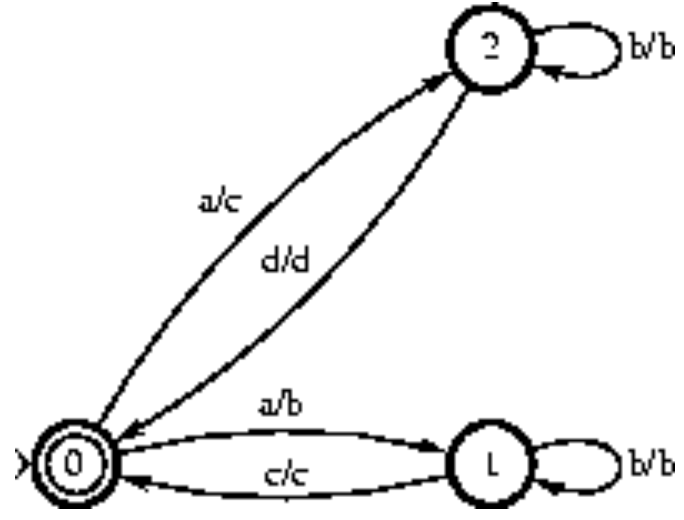
\includegraphics[scale=0.4]{nondetfst.png}
    \caption{Example of a non-deterministic FST that cannot be determinized.}
    \label{nondetfst}
\end{figure}

If the system is in state $0$ and it reads an $a$, then it can only decide which transition to take after reading an unbounded number of $b$'s. 
The algorithm enters an infinite loop for transducers for which no determinized version exists.


\section{Conclusion}

Finite-State Transducers derive from foundational models of computation and extend the capabilities of finite automata by introducing output transformations. 
Their theoretical basis is related to regular languages (Type 3 of Chomsky's hierarchy). We also explored the two main types of FSTs, Mealy and Moore machines,
which differ in how they produce output. Also explored their equivalence, minimization techniques. Also touched on the challenges of determinization and minimization of non-deterministic FSTs
by looking at a general definition of FST.
By understanding these concepts, it is now possible to delve into the specifics of FSTs and their applications, such as in the OFLAT application.


% \lipsum[1-100]
% \lipsum[1-700]
% \lipsum[1-700]
